
\chapter{递归结构和递归过程}

\section{什么是递归?}

什么是递归?对话《和声小迷宫》已经展示了:递归就是嵌套,各种各样的嵌套。这个概念很普通(故事里的故事,电影中的电影,画中的画,俄式洋娃娃中的俄式洋娃娃(甚至括号说明中的括号说明!)——这些还只是递归魅力中的一小部分)。然而,读者应该注意本章中“递归”的含义与第三章中的含义只是稍有关联。它们之间的关系在本章末会清楚的。

有时递归似乎与悖论很接近,例如递归定义。这样的定义可能会给粗心的人一种印象,即事物自己定义自己。那就会出现绕圈子了,而且即使不导致悖论,也会导致无穷回归。但事实上,一种递归定义(当正确给出时)永远不会导致无穷回归或悖论。这是因为递归定义从来不以某一事物自身来定义这一事物,而总是用比其自身简单一些的说法来定义这个事物。下面我给出一些关于递归定义的例子,我的意思很快就会更清楚了。

在日常生活中,递归出现的最常见方式之一就是:由于有另一项更简单的工作而拖延完成正在进行的一项工作(通常是同类型的工作)。这里有一个很好的例子。一个秘书有一部奇特的电话机,可以接许多电话。她正与A通话的时候,B打来电话。于是她对A说:“您不介意稍等一会儿吧?”当然她并不在乎A是否介意,她只是按一下电钮,转到B。现在C又打来电话。于是B也同样被耽搁了。照这样可以无限进行下去,但我们对此还是别过于热衷。假定和C的通话结束了,我们这位秘书“弹”回到B,继续刚才的通话。

这时,A坐在电话线的另一端,手指敲着桌子,听着电话里让人心烦的宛如背景音乐似的杂音,克制着自己的恼火……现在最平淡的情况是,与B的谈话顺利结束,这位秘书最终回到与A的通话中。但是很有可能在与B的通话恢复后,又有一个新加入者——D——打来电话。B则又一次被推入通话等待者的堆栈,而D得到了照顾。与D通完话之后,回到B,然后再回到A。这位秘书无疑是机械得要命——但我们却是在以最准确的方式来解释递归。

\section{推入、弹出和堆栈}

前面的例子里介绍了递归的一些基本术语——至少在计算机专家们的眼中是术语。这些术语就是推入、弹出和堆栈(或者,更准确地说,是下推堆栈),它们都是相互关联的。这些术语作为人工智能的早期语言之一——IPL语言的一部分,第一次出现于二十世纪五十年代后期。在对话中,读者已经遇到了“推入”和“弹出”。但我还是要做些详细说明。推入即是暂停目前正在进行的工作,记住在什么地方停下的——并开始一项新的工作。这项新的工作通常被认为是比前一项工作“低一个层次”。而弹出则与此相反——即结束这个层次的操作,在上一层暂停之处恢复操作。

但是,怎样才能准确记住你在每一个层次中停在什么地方呢?回答是:你把有关的信息存储在一个堆栈里。因此堆栈起着表格的作用,它使你了解这样一些事情:\pnum{1}在那些未完成的工作中,你是在何处被打断的(行话:“返回地址”),\pnum{2}在被打断处你要记住的有关事项(行话:“变量约束”)。当你弹回去恢复某项工作时,堆栈保存着你的“环境”(行话:“现场”),所以你不会感到丢掉了什么。在打电话的例子中,堆栈告诉你在每个不同的层次谁在等候,以及你们被打断时你们的谈话进行到了什么地方。

这里顺便说一下,“推入”、“弹出”和“堆栈”这几个词都来自自助餐厅中一摞托盘的视觉形象。通常在下面有一个弹簧,将最上面的托盘几乎保持在一个固定的高度。当你把一个托盘推到这摞托盘上时,这一摞就往下陷一点儿——而当你从那一摞上拿下一个托盘时,整个一摞又都往上弹一点儿。

再举一个日常生活中的例子。当你收听新闻广播时,常常会有这样的事情:新闻播音员把你转到一个外国记者那里。“现在请听赛利·斯瓦波利从英国皮费格发来的消息。”而赛利有一盘地方新闻报告人同某人会见的磁带,在介绍了一些背景情况之后,她开始播放录音带。“我是尼格尔·勘特瓦拉德。这里是皮费格郊外发生大抢劫的地方。我在与××谈话……”。现在你降了三个层次。也许这个被会见的人也会放一盘某次谈话的磁带。在实际新闻报道中,降三个层次这种事并不少见,但令人吃惊的是,我们几乎没有被悬置的感觉。我们在下意识中很容易地把握了回溯机制。这么简单,也许是因为每一个层次都与其它层次有着截然不同的味道。如果它们都相似,我们立刻就弄乱了。

关于更复杂的递归,本章前面的对话就是一个例子。在那个对话中,阿基里斯和乌龟在各个不同的层次中都出现了,有时作为角色出现在他们正在阅读的故事里。这时你可能对正在发生的事情有点糊涂,必须高度集中注意力,才可能弄明白。“咱们来看看,真正的阿基里斯和乌龟仍然在郝晕的直升飞机上;但是第二层次的阿基里斯和乌龟是在艾舍尔的某张画中——然后他们发现了一本书,并读了起来;所以《和声小迷宫》中在纹道上漫游的是第三层次的阿基里斯和乌龟。不,等一等——我在什么地方遗漏了一个层次……”要想把握对话中递归的回溯机制,你的意识中必须得有一个心理堆栈。(见\fig{26})

\begin{figure}
%\includegraphics{img_026.png}
\begin{tikzpicture}[scale=0.75,arrow decoration,
  SN/.style={decorate, decoration={snake,amplitude=.4mm,segment length=2mm}},
  every node/.style={inner sep=2pt,%
  font=\footnotesize\offinterlineskip\lineskip1pt\relax}]
\draw (0,0) -- (2,0)    node[midway, below, align=center] {郝晕的\\空中巢穴}
                        coordinate (A)
            -- ++(0,-2) node[midway, right, align=center] {读\\书}
                        coordinate (B)
            -- ++(2,0)  node[midway, below] {阿基里斯家}
                        coordinate (C)
            -- ++(0,-2) node[midway, right, align=left] {推喝\\入下\\露}
                        coordinate (D)
            -- ++(1.5,0)node[midway, below] {凹与凸}
                        coordinate (E);
\coordinate (F) at ($(E)+(1,0)$);
\draw   (F) -- ++(1.5,0)node[midway, below] {蜥蜴}
                        coordinate (G)
            -- ++(0,-2) node[midway, right, align=center] {下\\一\\层\\楼}
                        coordinate (H)
            -- ++(1.5,0)node[midway, below] {大雕的和声小迷宫}
                        coordinate (I)
            -- ++(0,2)  node[midway, left, align=center] {吃\\弹\\出\\锅\\酥}
                        coordinate (J)
            -- ++(1.5,0)node[midway, below] {蜥蜴}
                        coordinate (K)
            -- ++(0,2)  node[midway, left, align=left] {图\\画垂\\运直\\动于}
                        coordinate (L)
            -- ++(2,0)  node[midway, below] {乌龟家}
                        coordinate (M);
\path [postaction=decorate] (A) -- (B);
\path [postaction=decorate] (C) -- (D);
\path [postaction=decorate] (G) -- (H);
\path [postaction=decorate] (I) -- (J);
\path [postaction=decorate] (K) -- (L);
\draw[dashed] (G) -- (J) (C) -- (L) (A) -- ($(A-|M)+(.5,0)$);
\draw [SN] ($(E)+(0,.8)$) -- ($(E)-(0,.8)$)
           node[right,pos=.3, xshift=1] {堕};
\draw [SN] ($(F)+(0,.8)$) -- ($(F)-(0,.8)$)
           node[left, pos=.7, xshift=-1] {界};
\end{tikzpicture}
\caption[对话《和声小迷宫》的结构。]
  {对话《和声小迷宫》结构示意图。垂直下落是“推入”,上升是“弹出”。注意此图与对话中缩进格式的相似之处。从这个图可以清楚地看出最初的紧张——赫晕的恫吓——从未解决,阿基里斯和乌龟还在空中悬着。有些读者可能会为这个没弹出来的推入而备受折磨,而有些读者则可能眼都不眨。在这个故事里,巴赫的音乐迷宫也同样被过于迅速地截止——而阿基里斯甚至没有注意到任何怪异之处。只有乌龟意识到了那个全局性的由于悬搁而造成的紧张。}
\end{figure}

\section{音乐中的堆栈}

在谈及《和声小迷宫》时,我们应该讨论对话中没有明确说出,然而却暗示到的东西:我们递归地听音乐——特别是,我们保持一个关于调子的心理堆栈,每一个新的变调都把一个新的调子推上堆栈。进一步说,这就像是我们想听到调子以相反的顺序,从堆栈中一个一个地弹出,直到还原到主调音。这是个夸张,然而这里面也有一点道理。

任何有一定音乐修养的人都自动保持着一个装有两个调子的“浅堆栈”。在这个浅堆栈中,存放着真正的主调音和与之最接近的“伪主调”(即作曲家假装采用的那个调子)。也就是说,存放着最具“全局性”的调子和最具“局部性”的调子。这样,听众就可以知道什么时候回到了主调,并有一种强烈的“如释重负”的感觉。听众还可以区分(不像阿基里斯那样)局部性的松弛——例如,伪主调的解决——和全局性的解决。实际上,“伪解决”应该加强而不是松弛全局的紧张,因为它是一种嘲弄——就像阿基里斯尽管从“摇曳的灯”那个危险的处境脱险了,但我们都知道他和乌龟事实上正在郝晕先生的刀下等待着悲惨命运的到来。

紧张和解决是音乐的核心,因此这种例子非常之多。但我们只看两支巴赫的曲子。巴赫以“AABB”的形式写了许多曲子——即由两部分组成,每一部分都重复。我们来看看法国组曲第五号中的基格舞曲,这是一个典型的例子。它的主调是G调,我们听到一个欢快的舞曲旋律,它强烈地建立起G调。然而,A乐节中的变调把曲子引向非常接近的D调(第五度音)。A乐节结束时是在D调上。实际上这个曲子听起来好像以D调结束!(至少对阿基里斯来说可能是那样。)但这时一件奇怪的事情发生了——我们突然回到开始,回到G调,并重新听到向D调的转变。

然后是B乐节。由于乐曲主题的转位,我们从D开始,就好像D一直是主调似的,但我们最终还是回到G,就是说,我们弹回到主调。然后B乐节圆满地结束。随后,那个有趣的重复出现了,不加提醒地把我们猛拉回到D,并又一次让我们回到G。随后,那个有趣的重复出现了,不加提醒地把我们猛拉回到D,并又一次让我们回到G。

所有这些调子转换(有些是急剧的,有些是平稳的)的心理作用是很难描述的。这是音乐魔力的组成部分:我们能自动跟上这些转换。或者,也许是由于巴赫的魔力,他能够写出具有这样一种结构的曲子,这种结构如此自然优美,以至于我们根本弄不清究竟发生了什么。

《和声小迷宫》原作是巴赫的一支曲子。在这支曲子里,巴赫试图让听众在调子急剧变换的迷宫中迷失方向。很快,听众就晕头转向,没有任何方向感了——听众不知道真正的主调音在哪里。除非他有完美的乐感,或者像忒修斯(希腊神话中的雅典王子,曾进入克里特迷宫斩妖除怪的英雄)那样,有一个像阿里阿德涅(希腊神话中克里特王弥诺斯的女儿,曾给忒修斯一条线绳,使他得以走出迷宫)那样的朋友,给你一条线绳,使你得以顺原路返回。在这里,线绳应该是写出来的总谱。这部曲子展示出:作为音乐听众,我们没有极其可靠的、很深的堆栈。(另外一个例子是“无穷升高的卡农”)

\section{语言中的递归}

我们在语言上的心理堆栈能力也许稍强一点。所有语言的语法结构都涉及建立一个非常精细的下推栈,虽然,可以肯定,随着推进堆栈的次数的增加,理解一个句子的难度也急剧增大。语言中推入和弹出的极好例子就是那种反映在那些关于一位心不在焉地以使人心中的堆栈完全乱套的方式信口开河地使用使听众莫名其妙的相互叠套的动词或介词的教授的滑稽故事中的现象。想起这时在听众中造成的那种因为那些先前推入的教授所说的动词或介词在从栈中被弹出时其次序被搞乱而引起的的确确使人发笑混乱状态。但是在正常的口语中,几乎从未出现过如此深的堆栈——事实上,为了避免为维持堆栈做心理上的努力,说话的人经常要把复杂句子断成许多简单的句子。虽然每种语言都有涉及堆栈的结构,但大多不像上面那个例子那么突出,而且总是有重新组句的方法,以使堆栈的深度达到最低限度。

\section{递归迁移网}

句子的句法结构提供了一个好场所,以展示一种描述递归结构和过程的方式:递归迁移网(RTN)。RTN是一个图,它表示出为完成一项特殊任务可以遵循的各种通道。每个通道都包含几个结点——即里面有词的小方格——它们由带箭头的弧线连接起来。每个RTN的全名分开写在图的左边,第一个和最后一个结点里写有开始和结束。所有其它的结点里或者写有简单明了的操作说明,或者写有其它RTN的名称。每当碰到一个结点时,必须按照里面的说明去做,或者跳到这个结点所标明的那个RTN去。

我们来看一个RTN的例子——“花哨名词”。它告诉我们如何造出某种类型的名词短语。(见\fig{27}a)。如果我们完全水平地通过花哨名词,我们开始,然后造出一个指示代词、一个量词、一个形容词、再一个名词,然后结束。例如“那件愚蠢桌子”、“这只胖山谷”。但弧线也表示出其它可能性,例如,省略指示代词,或者重复形容词。这样就可以造出“牛奶”、“大红新喷嚏”等等。

\begin{figure}
%\includegraphics{img_027.png}
\tikzset{RE/.style={  arrow decoration,
  node distance=8mm and 8mm,
  every node/.style={draw, font=\small, inner sep=2pt}}}
\begin{subfigure}{\linewidth}\centering
\begin{tikzpicture}[RE]
\node[circle, inner sep=1pt] (A) {开始};
\node (B) [right= of A]{指示代词};
\node (C) [right= of B]{量词};
\node (D) [right= of C]{形容词};
\node (E) [right= of D]{名词};
\node[circle, inner sep=1pt] (F) [right= of E]{结束};
\path (A) edge[postaction=decorate] (B)
      (B) edge[postaction=decorate] (C)
      (C) edge[postaction=decorate] (D)
      (D) edge[postaction=decorate] (E)
      (E) edge[postaction=decorate] (F)
      (D) edge[postaction=decorate,
                below, out=320, in=215, loop, distance=5mm, ] (D);
\draw[rounded corners=10pt, postaction=decorate]
  (A) -- ($(A) + (5mm, 7mm)$) -- ($(D) + (-5mm, 7mm)$) -- (D.north);
\draw[rounded corners=10pt, postaction=decorate]
  (A) -- ($(A) + (5mm, 10mm)$) -- ($(E) + (-5mm, 10mm)$) -- (E.north);
\draw[rounded corners=10pt, postaction=decorate]
  (E.south) -- ($(E) - (5mm, 7mm)$) -- ($(C) + (5mm, -7mm)$) -- (C.south);
\end{tikzpicture}
\caption{花哨名词}
\end{subfigure}\par\bigskip
\begin{subfigure}{\linewidth}\centering
\begin{tikzpicture}[RE]
\node[circle, inner sep=1pt] (A) {开始};
\node (B) [above right= of A, xshift=2mm]{豪华名词};
\node (C) [right= of B]{及物动词};
\node (D) [right= of C]{\hbox{“的”\unskip}};
\node[anchor=west] (E) at ([xshift=4mm]D.east |- A) {花哨动词};
\node[circle, inner sep=1pt] (F) [right= of E]{结束};
\node (G) [below right = of A, yshift=5mm, xshift=2mm] {及物动词};
\node (H) [below right = of A, yshift=-5mm, xshift=2mm] {介词};
\node (I) at ({$(G)!.5!(H)$} -| C) {豪华名词};
\node (J) at (I -| D) {\hbox{“的”\unskip}};
\path (A) edge[postaction=decorate, bend left] (B.west)
          edge[postaction=decorate, bend right=15] (G.west)
          edge[postaction=decorate, bend right] (H.west)
          edge[postaction=decorate] (E)
      (B) edge[postaction=decorate] (C)
      (C) edge[postaction=decorate] (D)
      (D.east) edge[postaction=decorate, bend left] (E.north)
      (E) edge[postaction=decorate] (F)
      (I) edge[postaction=decorate] (J)
      (J) edge[postaction=decorate, bend right] (E.south);
\draw[rounded corners=5pt, postaction=decorate]
  (G) -| (I.north);
\draw[rounded corners=5pt, postaction=decorate]
  (H) -| (I.south);
\end{tikzpicture}
\caption{豪华名词}
\end{subfigure}
\caption{花哨名词与豪华名词的递归迁移网。}
\end{figure}

当碰到名词时,你要做的是用那个叫做“名词”的未知黑箱,从其名词库中取出名词。这用计算机术语来说叫“过程调用”,就是说,暂时让一个过程(这里是名词)进入控制,这个过程\pnum{1}做自己份内的事情(产生一个名词),然后\pnum{2}把控制权交还给你。上面的RTN里有四个这样的过程调用:指示代词、量词、形容词和名词。

花哨名词这一RTN本身又可以被其它RTN调用——比如,被叫做“句子”的RTN调用。在这个例子里,花哨名词会产生一个像“那件愚蠢桌子”这样的短语,然后回到句子中它曾被调出的地方。这倒使人想起在层层嵌套的电话、新闻报道中,恢复中断之处的方式!

然而,尽管我们称之为“递归迁移网”,到现在为止我们还没有展示任何真正的递归呢。当你进入一个像\fig{27}b那样的“豪华名词”RTN时,事情就变成递归的,而且似乎是循环的了。可以看出,在豪华名词中,每一条可行的通道都要调用花哨名词,所以无法避免地会得到一个这样或那样的名词。并且有可能不再带任何非花哨名词所提供的修饰语,而只是出现“牛奶”或者“大红新喷嚏”。不过有三条通道带有对豪华名词本身的递归调用。看起来当然就像事物自己定义自己了。是不是这样呢?

回答是“是,但却是一个良性的‘是’”。假如在过程句子中有一个结点叫做豪华名词,我们碰见了它。这意味着我们要在记忆(即堆栈)里设立这个结点在句子中的位置,以便知道返回到哪里——然后,我们把注意力转移到豪华名词过程上去。现在,为了生成一个豪华名词,我们必须选择一条通道。假定我们选择下边通道的上面一条通道——其调用顺序是:
\begin{center}
及物动词,豪华名词,的,花哨名词。
\end{center}
于是我们先吐出一个及物动词“结交”。下一个是要求我们给出一个豪华名词,可我们却恰好在豪华名词中间!是的,但不要忘记,我们的秘书也是在通话中间接到另一个电话的。她所做的只是把前一个电话的状态储存在一个堆栈里,然后开始打另一个电话,好像没有任何不寻常之处。下面我们也这样做。

首先我们在堆栈里写下我们在外层调用豪华名词时所在的那个结点,以便有一个“返回地址”,然后,就好像没有任何不寻常之处似的,我们弹回到豪华名词的开始处。现在我们得再选择一条通道。为了有点变化,这次我们选择底下那条:介词;豪华名词;的;花哨名词。这意味着产生一个介词(比如“朝向”),再产生一个豪华名词——我们又一次遇到了递归。于是我们停下来,再下降一个层次。为了避免复杂化,假定这次我们在豪华名词中选用的通道是直截了当的——就是个花哨名词。例如,我们因此得到的是“逻辑”。然后碰见的是此次调用豪华名词的终结之处,即结束这个结点,这等于是弹出来,于是我们到堆栈里去寻找返回地址。堆栈告诉我们,我们是在执行高一层次的豪华名词过程中间——所以我们从那里开始。这时我们的结果是“朝向逻辑”。在这一层次上,我们接下去碰见的是结点“的”,然后是结点花哨名词,比如说产生的是“鼻子”。至此,我们在这个层次上也达到了结点“结束”。于是我们又一次弹出。这时的结果是“结交朝向逻辑的鼻子”。我们在这最外层次上继续往下走,碰见的是结点“的”,然后结点花哨名词,我们设想由它产生的是“努力”。现在,我们到达了结点结束,这样我们就完成了对豪华名词的最外层调用,得到的是短语:
\begin{center}
“结交朝向逻辑的鼻子的努力”
\end{center}
我们最后一次弹出时,就把它传递给一直耐心等待的句子。

你也看到了,我们并没有陷入无穷回归。因为在RTN豪华名词里至少有一条通道不涉及任何对豪华名词本身的递归调用。当然,我们可以永远坚持选择豪华名词中的最下面一条通道,那么我们将永远无法结束,就像“\emph{造物神}”永远无法完全展开一样。但是,如果通道是任意选择的,就不会发生无穷回归。

\section{“终了”和异层结构}

区分开递归定义与循环定义的关键事实,是前者总会“终了”。定义中总是有某一部分避免了自指,因而构造一个满足该定义的对象的过程最后总会“终了”。

在RTN中还有比调用自身更为间接的达到递归的手段,即一个与艾舍尔的《画手》(\fig{135})很相似的机制,其中两个过程互相调用,而不是调用自己。比如,我们可以有一个叫做“小句”的RTN,由豪华名词和及物动词组成,就是说,当它需要为及物动词设定主语时,它调用豪华名词;反过来,豪华名词的上通道中前面的部分实际上就是个小句,也即在豪华名词中有通道要调用小句这个RTN。这就是间接递归的一个例子。这也让人想起说谎者悖论的两步形式。

不用说,也可以有三个过程循环地互相调用——如此等等。可以有一个RTN的大家族,互相缠绕在一起,发疯一般地互相调用或调用自己。程序的这种结构,即没有单独的“最高层次”或“控制器”,称作“异层结构”(与“分层结构”或“层次结构”相对)。我相信这个概念是来自沃伦·麦克库洛赫,早期的控制论专家之一,虔诚地研究大脑和心智的学者。

\section{扩展结点}

一种形象地考虑RTN的方法是:你沿着某个通道移动时,若碰到要调用一个RTN的结点,你便“扩展”那个结点,也就是说,用那个它所调用的RTN的小副本来代替它(见\fig{28})。然后,你就进入那个小RTN!当你从中弹出时,你自动地回到大图中恰当的位置。而在小RTN里你还可以动手制造出更小的RTN。由于你是在碰到这些结点时才扩展它们,这就避免了无穷的图,甚至当一个RTN调用自己时也没关系。

\begin{figure}
%\includegraphics{img_028.png}
\tikzset{RE/.style={  arrow decoration,
  node distance=8mm and 8mm,
  every node/.style={draw, font=\small, inner sep=2pt}}}
\sbox8{%
\begin{tikzpicture}[RE, line width=1.6pt, baseline=(I.south)]
\node[circle, inner sep=1pt] (A) {\phantom{开始}};
\node (B) [above right= of A, xshift=2mm]{\phantom{豪华名词}};
\node (C) [right= of B]{\phantom{及物动词}};
\node (D) [right= of C]{\phantom{\hbox{“的”\unskip}}};
\node[anchor=west] (E) at ([xshift=4mm]D.east |- A) {\phantom{花哨动词}};
\node[circle, inner sep=1pt] (F) [right= of E]{\phantom{结束}};
\node (G) [below right = of A, yshift=5mm, xshift=2mm] {\phantom{及物动词}};
\node (H) [below right = of A, yshift=-5mm, xshift=2mm] {\phantom{介词}};
\node (I) at ({$(G)!.5!(H)$} -| C) {\phantom{豪华名词}};
\node (J) at (I -| D) {\phantom{\hbox{“的”\unskip}}};
\path (A) edge[postaction=decorate, bend left] (B.west)
          edge[postaction=decorate, bend right=15] (G.west)
          edge[postaction=decorate, bend right] (H.west)
          edge[postaction=decorate] (E)
      (B) edge[postaction=decorate] (C)
      (C) edge[postaction=decorate] (D)
      (D.east) edge[postaction=decorate, bend left] (E.north)
      (E) edge[postaction=decorate] (F)
      (I) edge[postaction=decorate] (J)
      (J) edge[postaction=decorate, bend right] (E.south);
\draw[rounded corners=5pt, postaction=decorate]
  (G) -| (I.north);
\draw[rounded corners=5pt, postaction=decorate]
  (H) -| (I.south);
\end{tikzpicture}}
\sbox8{\scalebox{.25}{\copy8}}%
\edef\MYDEPTH{\the\dp8}%
\dp8=0pt\relax
\begin{tikzpicture}[RE, node distance=8mm and 7mm]
\node[circle, inner sep=1pt] (A) {开始};
\scoped[every node/.style={inner xsep=-3pt}]
  \node (B) [above right= of A, yshift=-3mm] {\copy8};
\node (C) [right= 6mm of B, xshift=1mm]{及物动词};
\node (D) [right= of C]{\hbox{“的”\unskip}};
\node[anchor=west] (E) at ([xshift=2mm]D.east |- A) {花哨动词};
\node[circle, inner sep=1pt] (F) [right= of E,xshift=-1mm]{结束};
\node (G) [below right = of A, xshift=2mm, yshift=5mm] {及物动词};
\node (H) [below right = of A, xshift=2mm, yshift=-5mm] {介词};
\node (I) at ({$(G)!.5!(H)$} -| C) {豪华名词};
\node (J) at (I -| D) {\hbox{“的”\unskip}};
\path (A) edge[postaction=decorate, bend left] (B.west)
          edge[postaction=decorate, bend right=15] (G.west)
          edge[postaction=decorate, bend right] (H.west)
          edge[postaction=decorate] (E)
      (B) edge[postaction=decorate] (C)
      (C) edge[postaction=decorate] (D)
      (D.east) edge[postaction=decorate, bend left] (E.north)
      (E) edge[postaction=decorate] (F)
      (I) edge[postaction=decorate] (J)
      (J) edge[postaction=decorate, bend right] (E.south);
\draw[rounded corners=5pt, postaction=decorate]
  (G) -| (I.north);
\draw[rounded corners=5pt, postaction=decorate]
  (H) -| (I.south);
\draw[dashed, thin] ($(B.south west) - (5pt,\MYDEPTH)$) rectangle
                    ($(B.north east) + (5pt,0)$);
\end{tikzpicture}
\caption{豪华名词的RTN,其中有一个结点递归地扩展了。}
\end{figure}

扩展结点有点像把首字组合的词中的字换成它所代表的词。词首字组合“\emph{造物神}”是递归的,但有个缺点——或者说是优点——你必须重复地扩展“\emph{造}”,这样就永远无法终了。不过,当RTN实现为一个实际的计算机程序时,总要有至少一条通道直接或间接地避免了递归,因此不会造成无穷回归。即使是最为典型的异层结构型程序也会终了——否则它无法运行!它会一个结点接一个结点不断地扩展,而永远不执行任何操作。

\section{图案G和递归序列}

无穷的几何结构可以用同样的方式来定义——就是一个结点一个结点地扩展。比如,我们来定义一个无穷的图案,称作“图案G”。我们用隐含表示法进行定义:在两个结点上标上字母G,用它代表整个图案G的一个副本。在\fig{29}a中,图案G是隐含地描绘的。如果我们想更清楚地看到图案G,就扩展那两个G——即代之以同样的图案,只是规模缩小了(见\fig{29}b)。图案G的这个二阶版本提示给我们那个最终的、不可能实现的图案G实际上是个什么样。\fig{30}显示出了更大部分图案G的,其中所有的结点都从下到上从左到右地标上了数字。两个额外的结点——数字1和2——插在了底部。

\begin{figure}
%\includegraphics{img_029.png}
\tikzset{RE/.style={%
  every node/.style={draw, circle, fill=black,
    inner sep=0pt, minimum size=3pt},
  end/.style={every node/.style={inner sep=2pt}},
  grow'=up, level distance=4mm,
  level 1/.style={sibling distance=25mm},
  level 2/.style={sibling distance=12.5mm},
  edge from parent path={%
    let \p1= (\tikzchildnode\tikzchildanchor),
        \p2= (\tikzparentnode\tikzparentanchor) in
    \pgfextra{\tikzxtest}
    (\tikzparentnode\tikzparentanchor)
    \tikzxtestresult { -- } { -| }
    (\tikzchildnode\tikzchildanchor)}}}
\floatsetup{heightadjust=none}
\begin{lrbox}{\TEMPBOX}
\begin{tikzpicture}[RE]
\node (a) {}
  child [end] { node {G} }
  child { node {}
    child [end] { node {G} }
  };
\draw (a) -- +(0,-3mm);
\end{tikzpicture}
\end{lrbox}
\begin{lrbox}{4}
\begin{tikzpicture}[RE]
\node (a) {}
  child [end] { node {H} }
  child { node {}
    child { node {}
      child [end] { node {H} }
    }
  };
\draw (a) -- +(0,-3mm);
\end{tikzpicture}
\end{lrbox}
\begin{lrbox}{6}
\begin{tikzpicture}[RE]
\node (a) {}
  child { node {}
    child [end] { node {G} }
    child { node {}
      child [end] { node {G} }
    }
  }
  child { node {}
    child { node {}
      child [end] { node {G} }
      child { node {}
        child [end] { node {G} }
      }
    }
  };
\draw (a) -- +(0,-3mm);
\end{tikzpicture}
\end{lrbox}
\begin{lrbox}{8}
\begin{tikzpicture}[RE]
\node (a) {}
  child { node {}
    child [end] { node {H} }
    child { node {}
      child { node {}
        child [end] { node {H} }
      }
    }
  }
  child { node {}
    child { node {}
      child { node {}
        child [end] { node {H} }
        child { node {}
          child { node {}
            child [end] { node {H} }
          }
        }
      }
    }
  };
\draw (a) -- +(0,-3mm);
\end{tikzpicture}
\end{lrbox}
\figurebox[\textwidth]{%
  \begin{subfloatrow}
    \figurebox{\usebox\TEMPBOX}{\caption{图案G,未扩展。}}
    \figurebox{\usebox4}{\caption{图案H,未扩展。}}
  \end{subfloatrow}\par
  \begin{subfloatrow}
    \figurebox{\usebox6}{\caption{图案G,扩展一次。}}
    \figurebox{\usebox8}{\caption{图案H,扩展一次。}}
  \end{subfloatrow}}
{\caption{隐含表示的图案G和图案H。}}
\end{figure}

\begin{figure}
%\includegraphics{img_030.png}
\begin{tikzpicture}[%
  every node/.style={draw, circle, font=\small,
    inner sep=0pt, minimum size=11pt},
  grow'=up, level distance=6mm,
  level 3/.style={sibling distance=46.5mm},
  level 4/.style={sibling distance=27mm},
  level 5/.style={sibling distance=18mm},
  level 6/.style={sibling distance=12mm},
  edge from parent path={%
    let \p1= (\tikzchildnode\tikzchildanchor),
        \p2= (\tikzparentnode\tikzparentanchor) in
    \pgfextra{\tikzxtest}
    (\tikzparentnode\tikzparentanchor)
    \tikzxtestresult { -- } { -| }
    (\tikzchildnode\tikzchildanchor)}]
\node {1}
child { node {2}
  child { node {3}
    child { node {4}
      child { node {6}
        child { node {9}
          child { node {14} }
          child { node {15} }
        }
        child { node {10}
          child { node {16} }
        }
      }
      child { node {7}
        child { node {11}
          child { node {17} }
          child { node {18} }
        }
      }
    }
    child { node {5}
      child { node {8}
        child { node {12}
          child { node {19} }
          child { node {20} }
        }
        child { node {13}
          child { node {21} }
        }
      }
    }
  }
};
\end{tikzpicture}
\caption[进一步扩展了的图案G。]
  {图案G,进一步地扩展了,并为结点标了数字。}
\end{figure}

这棵无穷树有着非常奇特的数学性质。从右边往上数是著名的斐波那契数列:
\[
\begin{tikzpicture}[inner sep=0pt]
\matrix [matrix of math nodes, column sep=7pt, anchor=base]
  {
     1, & 1, & 2, & 3, & 5, & 8, & 13, &
    21, & 34, & 55, & 89, & 144, & 233, & \dotsc \\
  };
\end{tikzpicture}
\]
这是由比萨的列奥那多于1902年发现的,他是波那契奥[Bonaccio]的儿子,因此叫“斐利尤斯·波那契”[Filius Bonacci,拉丁语,意即波那契奥之子]或简称“斐波那契”。这些数可由一对方程极好地递归定义出来:
\begin{align*}
\fibo(n) & =\fibo(n-1)+\fibo(n-2) \quad \text{当$n>2$} \\
\fibo(1) & =\fibo(2)=1
\end{align*}
注意新的斐波那契数是如何用前面的斐波那契数定义的。我们可以在RTN中表示这组方程(见\fig{31})。

\begin{figure}
%\includegraphics{img_031.png}
\begin{tikzpicture}[arrow decoration,
  node distance=8mm, every node/.style={font=\small, inner sep=2pt},
  fm/.style={draw,minimum height=\ht\strutbox}]
\node [draw, circle, inner sep=1pt] (A) {开始};
\node [left= 1mm of A] {$\fibo(n)$: };
\node[fm] (C) [above= 4mm of A, xshift=12mm, anchor=west]{令$x=\fibo(n-1)$};
\node[fm] (B) [above= 5mm of C]{令$y=\fibo(n-2)$};
\node[fm] (D) [right= 10mm of C]{$x+y$};
\node[draw, circle, inner sep=1pt] (E) at ([xshift=15mm]D.east |- A){结束};
\node[fm] (F) at ([yshift=-8mm]$(A)!.5!(E)$){值是$1$};
\path (B) edge[postaction=decorate] (C)
      (C) edge[postaction=decorate] (D);
\path [postaction=decorate] (A) -- ( A |- B);
\draw[rounded corners=10pt]
  (A) |- (B) node[pos=.4,left,font=\footnotesize] {若$n>2$};
\draw[rounded corners=10pt, postaction=decorate]
  (D) -| (E);
\draw[rounded corners=10pt, postaction=decorate]
  (A) |- (F) node[near end,below,font=\footnotesize] {若$n=1$或$2$};
\draw[rounded corners=10pt, postaction=decorate]
  (F) -| (E);
\end{tikzpicture}
\caption[斐波那契数的RTN。]
  {一个斐波那契数的递归迁移网。}
\end{figure}

这样,要想计算$\fibo(15)$,就可以对上面RTN定义的过程进行一系列的递归调用。你随着下降的$n$值倒推到$\fibo(1)$或$\fibo(2)$(已显明地给出了),这个递归定义就终止了。这种倒推的计算方法有点笨拙,其实你可以很容易地从$\fibo(1)$和$\fibo(2)$开始,一直向前推:不断地加上最新的两个值,直到$\fibo(15)$。这样的话你就无须对堆栈进行回溯了。

图案G还有一些比这更令人惊异的性质。它的整个结构可以仅用一个递归定义来编码,如下所示:
\begin{align*}
\mG(n) & = n-\mG(\mG(n-1)) \quad \text{当$n>2$} \\
\mG(0) & = 0
\end{align*}

函数$\mG(n)$是如何为前述树结构编码的?很简单。对每个$n$算出$\mG(n)$,并把计算结果放在$n$下面以构成一棵树,就可以重新建立起图案G。事实上,最初我就是这么发现图案G的。我在研究函数$\mG(n)$的时候,试图很快地计算它的值,我想到了把已知的值表示成一棵树。使我惊讶的是,这棵树最后竟会有这种极其规则的递归几何描述。

更奇妙的是,假如为比$\mG(n)$多一层嵌套的函数$\mH(n)$——
\begin{align*}
\mH(n) & = n-\mH(\mH(\mH(n-1))) \quad \text{当$n>2$} \\
\mH(0) & = 0
\end{align*}
——构造一个类似的树,那么相关的“图案H”就隐含地定义出来了,如\fig{29}c。唯一不同的是右边的一枝多出一个结点。图案H的第一个递归扩展在\fig{29}d中给出。而对任意深度的嵌套也都是如此。递归几何结构有着优美的规则性,恰好与递归代数结构相对应。

好奇的读者可以考虑一下这个问题:假设你把图案G翻转——就像出现在镜子里那样——然后自左向右地对这棵新的树中的结点进行标号。那么,对于这棵“翻转的树”,你是否能找到一个递归的代数定义?H树的“翻转”又如何?其它的呢?

另一个有趣的问题是关于一对递归地交织在一起的函数$\mF(n)$和$\mM(n)$——可以说是“联姻”的两个函数。它们是这样定义的:
\begin{gather*}
\left.
\begin{aligned}
\mF(n) & = n-\mM(\mF(n-1)) \\
\mM(n) & = n-\mF(\mM(n-1))
\end{aligned}
\enskip\right\} \quad \text{当$n>0$} \\
\mF(0)=1 \quad \text{而} \quad \mM(0)=0
\end{gather*}
这两个函数的RTN彼此互相调用,同时也调用它们自己。问题只是去发现图案F和图案M的递归结构。它们非常优美而且简单。

\section{一个紊乱的序列}

我们关于数论中的递归的最后一个例子稍有点神秘。请考虑下面这个递归的函数定义:
\begin{align*}
\mQ(n) & = \mQ(n-\mQ(n-1))+\mQ(n-\mQ(n-2)) \quad \text{当$n>2$} \\
\mQ(1) & = \mQ(2)=1
\end{align*}

它使人想起斐波那契数的定义,在那里每一个新的值都是前面两个值的和——但这里不是紧挨着的前两个数的值。在这里,紧挨着的那前两个值是说明:往前数多少位,才能得到计算新值所要加起来的那两个数。前$17$个$\mQ$数排列如下:
\[
\begin{tikzpicture}[inner ysep=3pt, inner xsep=0pt, baseline=(E.north)]
\matrix [matrix of math nodes, column sep=7pt, anchor=base]
  {
    1, & 1, & 2, & 3, & 3, & 4, & 5, &
    |(a)| 5, &
    |(b)| 6, &
    6, & 6, & 8, & 8, & 8, & 10, &
    |(c)| 9,  &
    |(d)| 10, &
    \dotsc \\
  };
\begingroup
\settowidth\linewidth{$,$}
\divide \linewidth 2\relax
\edef\x{\endgroup
  \noexpand\node (A) [below= 8pt of a, xshift=-\the\linewidth] {$5$};
  \noexpand\node (B) [below= 8pt of b, xshift=-\the\linewidth] {$6$};
}\x
\draw[->] (A) -- (A |- a.south);
\draw[->] (B) -- (B |- b.south);
\node at ($(A)!.5!(B)$) {$+$};
\node (C) [right=0pt of B] {${}=\vphantom{1}$};
\node (D) [right=0pt of C] {$11$};
\node (E) [below=3pt of D, font=\footnotesize] {新值};
\draw[decorate,decoration=brace]
  (E.north west) -- (E.north east);
\draw[decorate,decoration=brace]
  (d.south east) -- (c.south west)
  node [midway, below=3pt, font=\footnotesize] {向左移多少位};
\end{tikzpicture}
\]
要得到下一个数,向左(从省略号开始)分别数$10$个数和$9$个数,遇到$5$和$6$,如箭头所示。它们的和——$11$——给出了$\mQ(18)$这个新值。在这个奇怪的过程里,已知的一列$\mQ$数被用来扩展自身。这样得到的序列,如果温和点说,是杂乱无章的。走得越远,它变得越没有意义。这是那些非常奇特的情况之一,即一个多少是个自然的定义,导致一个令人极度困惑的现象:以很有秩序的方式制造出了混乱。人们很自然地会想到:表面上的混乱是否隐含着某种微妙的规律性。当然,根据定义是有规律性的。但有趣的是,是否有另一种刻划这个序列的方式——要是运气好的话,最好一个非递归的定义。

\section{两个令人惊异的递归图}

数学里奇特的递归是不胜枚举的,而我的目的并不是把它们一一列举出来。不过,在我自己的经历中有两个特别触目的例子,值得把它们提出来。两个都是图形。一个出现在某些关于数论的研究里,另一个出现在我的博士学位论文——固体力学之中。最有趣的是这两个图形有着密切的联系。

\begin{figure}

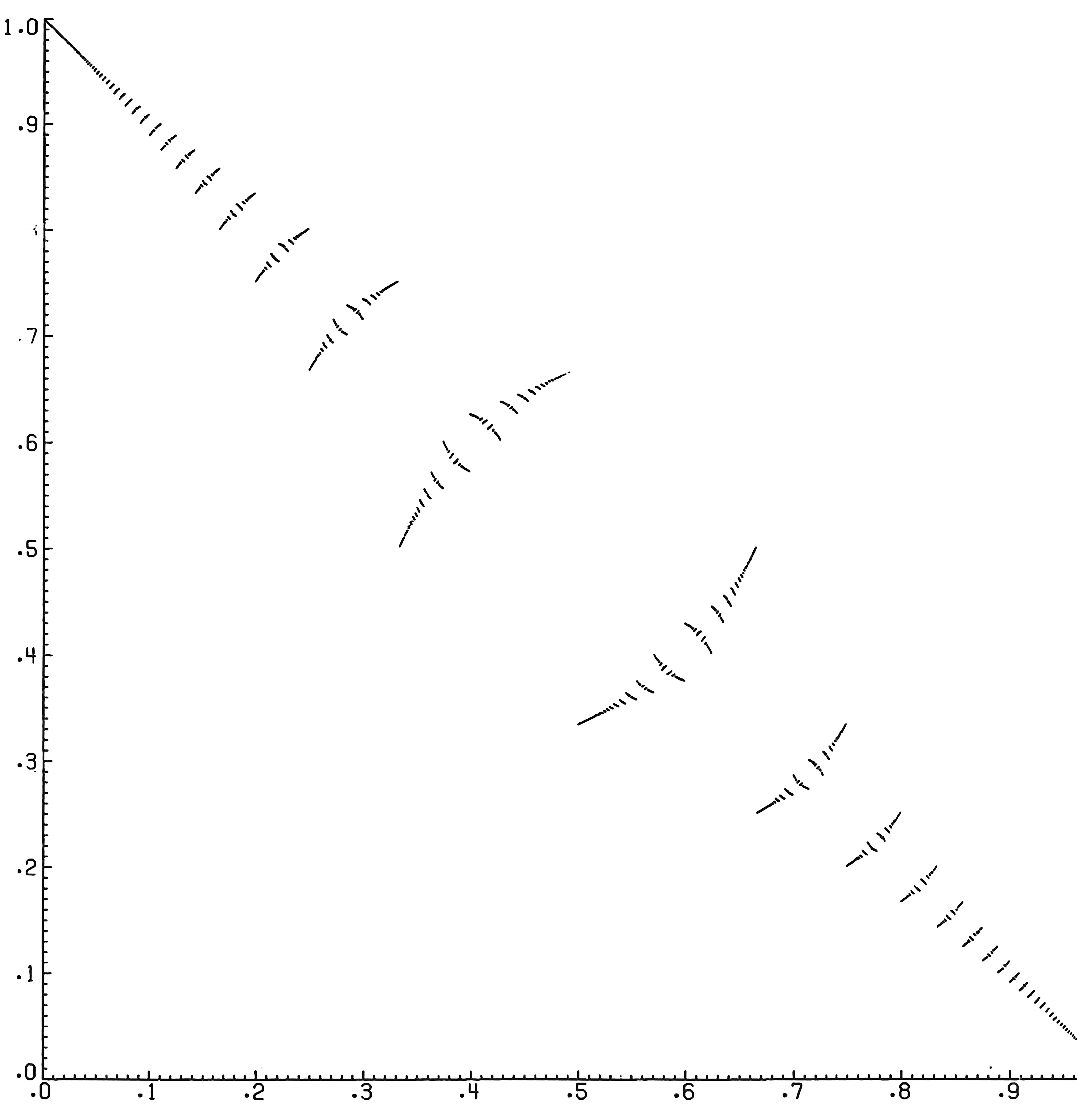
\includegraphics{img_032.png}
\caption[函数$\INT(x)$的图形。]
  {函数$\INT(x)$的图形。在$x$的每个有理数值处都是个跳跃性的不连续点。}
\end{figure}

第一个图形(\fig{32})是一个函数的图形,这函数我称为$\INT(x)$。这里给出的是$x$处于$0$和$1$之间的情形,对于$x$处于其它任意一组整数$n$和$n+1$之间的情形,你只要找到$\INT(x-n)$,然后再加上$n$即可。你可以看到,这个图的结构是跳跃式的,由无数个弯曲的片段组成。这些片段离角落越近就越小——并且也越直。假如你仔细观察每个这样的小片段,你会发现实际上它是整个图形的一个副本,只是弯曲了!这意味着丰富的内容。其中之一是:$\INT$图恰恰是由它本身的一个个副本组成的,它们层层嵌套,以至无穷。如果你拿出图的一小部分,不管是多小的一部分,你其实是拿着整个图形的一个完整的副本——事实上,是无穷多个副本!

$\INT$不是由别的,而是由它本身的一个个副本组成的,这一事实可能使你觉得它一定是短命的。它的定义似乎是循环的。它究竟是怎么开始的呢?这是件很有趣的事。最值得注意的是:如果向一个没见过$\INT$的人描述它那么仅仅说“它是由它本身的副本组成的”是不够的。事情的另一半——非递归的那一半——说明这些副本存在于正方形中的哪个地方、相对于整个图形它们是怎么变形的。只有把$\INT$的这两个方面结合起来,才能说明$\INT$的结构。这正像在斐波那契数的定义中一样,需要两条线索——一条线索定义递归,另一条定义“基底”(也就是最开始的值)。说得具体些就是:如果你设基础的值是$3$而不是$1$,就会产生完全不同的序列,即卢卡斯序列:
\[
\begin{tikzpicture}[inner ysep=3pt, inner xsep=0pt, baseline=(O.center)]
\matrix [matrix of math nodes, column sep=7pt, anchor=base]
  {
    |(a)| 1, &
    |(b)| 3, &
    4, & 7, & 11, & 18, &
    |(c)| 29, &
    |(d)| 47, &
    |(e)| 76, &
    123, & \dotsc \\
  };
\begingroup
\settowidth\linewidth{$,$}
\divide \linewidth 2\relax
\edef\x{\endgroup
  \noexpand\node (C) [below= 3pt of c, xshift=-\the\linewidth] {$29$};
  \noexpand\node (D) [below= 3pt of d, xshift=-\the\linewidth] {$47$};
  \noexpand\node (E) [below= 3pt of e, xshift=-\the\linewidth] {$76$};
}\x
\node at ($(C)!.5!(D)$) {$+$};
\node at ($(D)!.5!(E)$) {${}=\vphantom{7}$};
\draw[decorate,decoration=brace]
  (b.south east) -- (a.south west)
  node [midway, below=3pt, font=\footnotesize] {基底};
\node [below= 0pt of D, font=\linespread{1.2}\footnotesize, align=center]
  (O) {与斐波那契序列\\相同的递归规则};
\end{tikzpicture}
\]

在$\INT$的定义中,与基底相对应的是一个由许多小方框组成的图(\fig{33}a),它表示出副本在什么地方,它们是如何扭曲的。我们把它叫做$\INT$的“骨架”。从骨架开始构造$\INT$,需按下列步骤:首先,对于骨架的每个方框,你要做两件事:\pnum{1}把骨架的一个弯曲了的小副本放进方框,用里面的弯曲的线作为它的向导;\pnum{2}涂掉外面的方框及其弯线。一旦把原骨架的每一个方框都这样做了,每个大骨架原来所在之处就换成了许多的“小辈”骨架。下一步,降一个层次对那些小辈骨架重复这一过程。然后再重复,再重复,再重复……这样下去的极限就是$\INT$图,当然极限是达不到的。就这样,一层一层地把骨架嵌套于它自身之中,$\INT$图就“无中生有”地逐渐构造出来了。但事实上,这“无”不是虚无——是一幅图。

\begin{sidewaysfigure}
\figurebox[\linewidth]
  {%
    \begin{subfloatrow}
      \figurebox{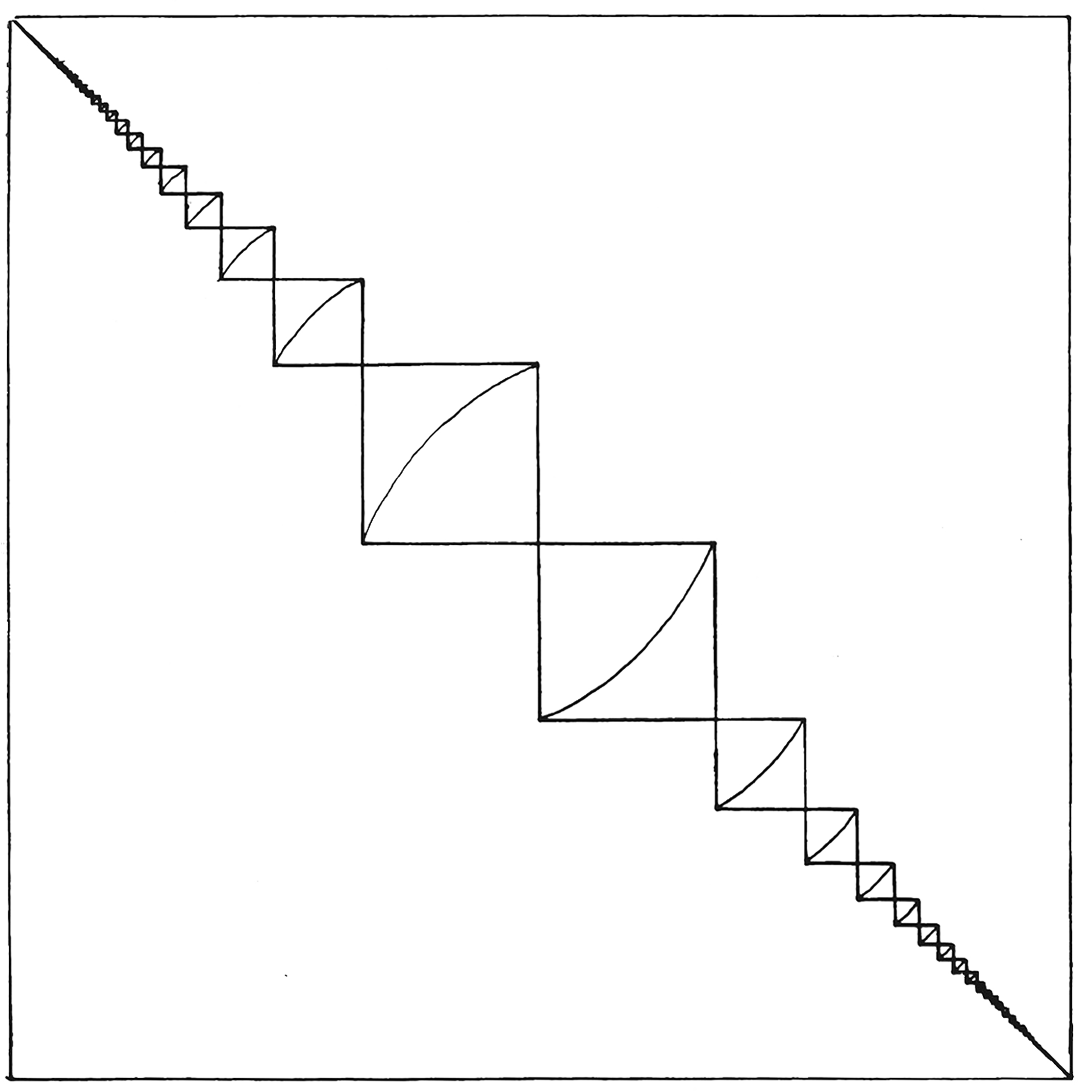
\includegraphics{img_033a.png}}
                {\caption{能用递归替换构造$\INT$的骨架。}}
      \figurebox{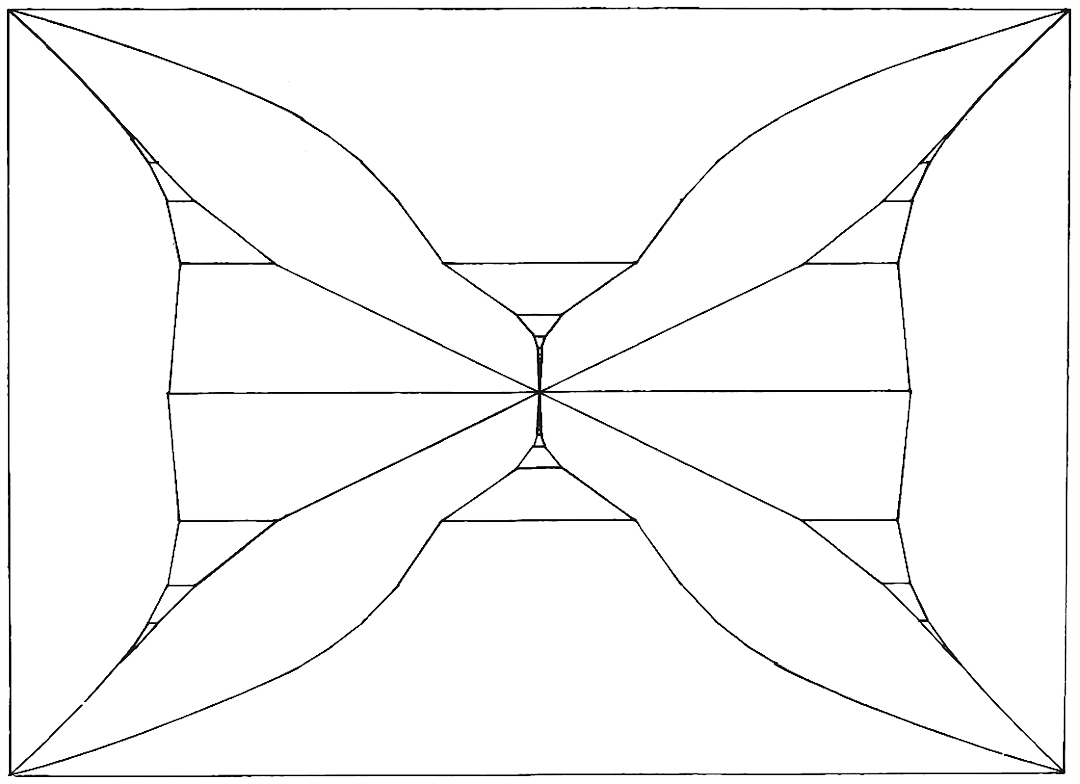
\includegraphics{img_033b.png}}
                {\caption{能用递归替换构造G图的骨架}}
    \end{subfloatrow}%
  }
  {\caption{$\INT$和G图的骨架。}}
\end{sidewaysfigure}

为了更清楚地看到这一点,可以设想保持$\INT$定义的递归部分,而改变其初始的图,即骨架。改变了的骨架如\fig{33}b中所示,同样是越接近四个角,方框就越小。如果你把这第二种骨架也一遍一遍地嵌套在它自身之中,就会得出我博士论文中那个关键的图,我称之为G图(\fig{34})(事实上,在每个副本上也还需要做些复杂的变形——但嵌套是基本思想)。这样,G图就是$\INT$家族中的一个成员了。它是个“远亲”,因为它的骨架和$\INT$的截然不同,也复杂得多。然而,递归的部分是一样的,“亲族关系”体现在这里面。

\begin{figure}
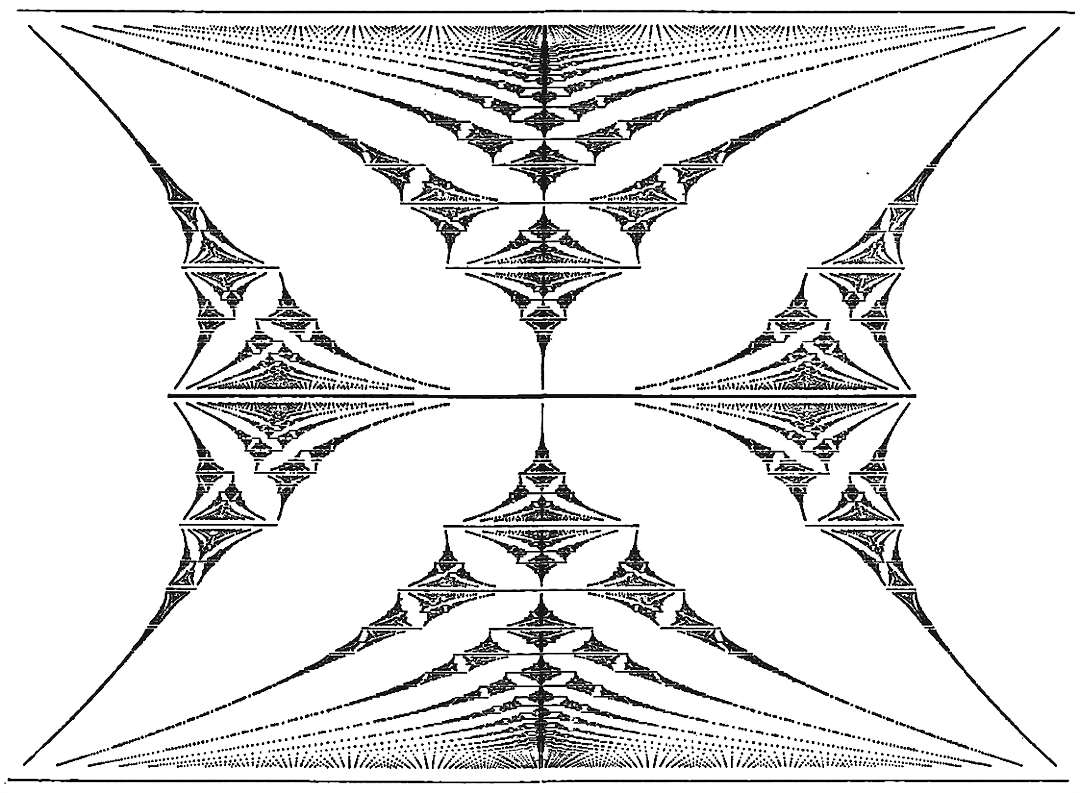
\includegraphics{img_034.png}
\caption[G图:一个递归图形。]
  {G图:一个递归图形,显示了一个磁场中理想晶体里的电子的能量带。$\alpha$代表磁场强度,沿垂直方向从0到1。能量是沿水平方向的。水平的线段是所允许的电子能量带。}
\end{figure}

我不该让读者到现在还不知道这些美丽图案的由来。$\INT$——代表“交换”——是来自一个涉及了“埃塔序列”的问题,与连分数有关。$\INT$的基本思想是加号与减号在某种连分数中互相转换。作为一个推论,我们有$\INT(\INT(x))=x$。$\INT$有一个性质,即:如果$x$是有理数,则$\INT(x)$也是;如果$x$是二次的,则$\INT(x)$也是二次的。我不知道这种趋向对于更高阶的代数度是否也成立。$\INT$的另外一个可爱的性质是:在$x$的全部有理数值上,它是跳跃的,不连续的,但在x的所有无理数值上,它是连续的。

G图来自一个问题的高度理想化形式,这个问题是:“磁场中晶体的容许电子能是什么?”这是个很有趣的问题,因为它交织了两个非常简单而又基本的物理现象:完全晶体中的电子,和均匀磁场中的电子。这两个比较简单的问题都得到了充分的理解,它们各自的典型解法似乎是彼此不相容的。因此,看看自然如何把它们调和起来,这将会是很有意思的。结果表明,没有磁场的晶体与没有晶体的磁场的确是有一个共同特征的:在两种情形中,电子都表现出周期性。于是,当两种情形合并在一起时,两个周期的比是个很关键的参数。事实上,这个比率包含了有关容许电子能分布的全部信息——但是,只有展开成连分数时,它才透露它的这一秘密。

G图显示出了这个分布。水平轴代表能量,垂直轴代表上面提到的周期比率,我们可以称之为“$\alpha$”。在底部,$\alpha$是$0$。在顶部,$\alpha$是$1$。当$\alpha$为$0$时,没有磁场。每一条构成G图的线段是一个“能量带”——就是说它代表能量的容许值。以大小不同的规模横穿G图的空白地带则是能量值的禁区。G图的一个惊人的性质是:当$\alpha$是有理数时(比如说是简约后的$p/q$),就恰好有$q$个这样的能量带(虽然当$q$是偶数时,有两个带在中间相遇)。当$\alpha$是无理数时,这些带则缩小成点,无数多个点,稀疏地分布在所谓“康托尔集”上——那是拓扑学中出现的另一种递归定义的东西。

你可能很想知道,在一个实验中,这样一个复杂的结构是否会出现。坦率地说,如果G图在什么实验里出现了,我会是这个世界上最为惊异的人。G图的物理意义在于:它指出了对这一类理想化程度较低的问题进行适当的数学处理的途径。换句话说,G图只是对理论物理的贡献,它无法对做实验的人提示什么可能看到的东西。我的一个持不可知论的朋友曾被G图的无穷多个无穷所震惊,于是把它叫做“上帝的画像”,我不认为这是亵渎神圣。

\section{物质最低层次上的递归}

我们在语言的语法中看到了递归,我们看到了永远向上生长的递归几何树,我们也看到了一种把递归引入固体物理学理论的方法。现在我们来换一种眼光,在这种眼光下,整个世界都是建立在递归之上的。这涉及到了基本粒子的结构:电子、质子、中子、以及被称作“光子”的微小的电磁辐射量子。我们将看到,粒子——精确的说法要用到相对论量子力学——是彼此嵌套的,对之可用递归来描述,甚至可用某种“语法”来描述。

我们的起点是这样一个事实:假如粒子不相互作用,那么一切都将是难以置信地简单。物理学家会喜欢这样的世界,因为这样一来,他们就可以很容易地计算出所有粒子的行为(这种世界里是否还有物理学家是可怀疑的)。没有相互作用的粒子叫做“裸粒子”。它们纯粹是假设的东西,并不实际存在。

当相互作用的“开关”被“打开”时,粒子就像函数$\mF$和$\mM$、或者说两个结了婚的人那样纠缠在一起。这些实际的粒子称为“重正化了的”——一个丑陋但却有启发性的术语。结果是,一个粒子如果不涉及所有其它粒子就无法给出定义,而其它粒子的定义反过来又要靠最初那个粒子,等等。这样转来转去,构成了一个永不停止的循环。

让我们更具体一点。我们只限于讨论两种粒子:电子和光子。不过还要附带上电子的反粒子——正电子(光子的反粒子是它自己)。首先,设想一下在一个乏味的世界中裸电子要从A点传到B点,就像芝诺在我那《三部创意曲》里所做的那样。一个物理学家会画出这样一个图:
\begin{center}
%\includegraphics{img_035-1.png}
\begin{tikzpicture}
\begin{feynman}
\vertex (a);
\vertex[right=5cm of a] (b);
\diagram* {
  (a) --[fermion] (b)
};
\fill (a) circle (.5mm);
\fill (b) circle (.5mm);
\end{feynman}
\end{tikzpicture}
\end{center}

有一个数学表达式与这条线及其端点相对应,而且很容易写下来。物理学家可以用这个表达式来理解裸电子在这个轨道上的行为。

现在让我们“打开”电磁相互作用的开关,让电子和光子相互作用。虽然光子没出现,还是有一些很有价值的结果,即使是在这么简单的轨道上。特别是,我们的电子现在变得能够放射、吸收“虚光子”——出现之后还未被看到就消失掉的光子。我们这样表示这个过程:
\begin{center}
%\includegraphics{img_035-2.png}
\begin{tikzpicture}
\begin{feynman}
\vertex (a);
\vertex[right=5cm of a] (b);
\vertex[right=1cm of a] (c);
\vertex[left=1cm of b] (d);
\diagram* {
  {[edges=fermion]
    (a) -- (c) -- (d) -- (b)
  },
  (c) --[photon, half left] (d)
};
\fill (a) circle (.5mm);
\fill (b) circle (.5mm);
\end{feynman}
\end{tikzpicture}
\end{center}
当我们的电子传播时,它可以一个接一个地放射和再吸收光子,它甚至可以嵌套这一过程,如下所示:
\begin{center}
%\includegraphics{img_035-3.png}
\begin{tikzpicture}
\begin{feynman}
\vertex (a);
\vertex[right=5cm of a] (b);
\vertex[right=1cm of a] (c);
\vertex[left=1cm of b] (d);
\vertex[right=.7cm of c] (e);
\vertex[left=.7cm of d] (f);
\diagram* {
  {[edges=fermion]
    (a) -- (c) -- (d) -- (b)
  },
  (c) --[photon, half left] (d),
  (e) --[photon, half left] (f)
};
\fill (a) circle (.5mm);
\fill (b) circle (.5mm);
\end{feynman}
\end{tikzpicture}
\end{center}
与这些图案——“费因曼图案”——相对应的数学表达式很容易写下来,但它们比裸电子的表达式难计算一些。真正使事情复杂化的是光子(实的或虚的)能在瞬间里衰变成一对正负电子。然后这一对电子相互湮灭,原来的光子魔术般又出现了。下面是这种过程的示意:
\begin{center}
%\includegraphics{img_035-4.png}
\begin{tikzpicture}
\begin{feynman}
\vertex (a);
\vertex[right=5cm of a] (b);
\vertex[right=15mm of a] (c);
\vertex[left=15mm of b] (d);
\diagram* {
  (a) --[photon] (c),
  (d) --[photon] (b),
  (c) --[fermion, half left] (d),
  (d) --[fermion, half left] (c)
};
\end{feynman}
\end{tikzpicture}
\end{center}
电子有一个指向右边的箭头,而正电子的箭头是指向左边。

读者或许已经预料到,这些虚的过程可以嵌套到任意深度。这可以产生出一些看起来非常复杂的图案,如\fig{35}。在费因曼图案中,一个电子从A的左边进入,演出一些惊人的杂技,之后一个电子在B的右边出现。对于一个看不出内情的观察者,似乎是一个电子从A平平安安地滑行到B,没有那些内部的混乱。在图案中,读者可以看到电子的曲线是怎样被随意地装饰,光子也是一样。要计算这个图案是非常之困难的。

\begin{figure}
%\includegraphics{img_035-5.png}
\begin{tikzpicture}
\begin{feynman}
\vertex[label=left:A] (a);
\vertex[right=15mm of a] (b);
\vertex[right=15mm of b] (c);
\vertex (d) at ($(c)+(-60:12mm)$);
\vertex (e) at ($(d)+(-120:15mm)$);
\vertex (f) at ($(e)+(-60:15mm)$);
\vertex[right=8mm of f] (g);
\vertex[right=8mm of g] (h);
\vertex (i) at ($(h)+(45:8mm)$);
\vertex (j) at ($(i)+(-45:8mm)$);
\vertex[right=8mm of j] (k);
\vertex[right=15mm of k, label=right:B] (l);
\vertex[above=8mm of i] (m);
\vertex (n) at ($(m)+(45:8mm)$);
\vertex (o) at ($(n)+(135:8mm)$);
\vertex (p) at ($(o)+(-135:8mm)$);
\vertex (q) at ($(d)+(-60:15mm)$);
\vertex[left=4mm of q] (r);
\vertex[right=4mm of q] (s);
\vertex[above=6mm of q] (t);
\vertex[below=6mm of q] (u);

\diagram* {
  {[edges=fermion]
    (a) -- (b) -- (c) -- (d) -- (e)
        -- (f) -- (g) -- (h) -- (i)
        -- (j) -- (k) -- (l)
    (m) -- (n) -- (o) -- (p) -- (m)
    (t) --[bend right] (r)
    (u) --[bend right] (s)
  },
  {[edges=photon]
    (b) -- (e),
    (m) -- (i),
    (n) -- (p),
    (r) -- (s),
    (d) -- (t),
    (u) -- (f),
    (c) --[bend left=75] (o),
    (h) --[half right] (j),
    (g) --[half right] (k)
  },
  (r) --[bend right] (u),
  (s) --[bend right] (t),
};
\fill (a) circle (.5mm);
\fill (l) circle (.5mm);
\end{feynman}
\end{tikzpicture}
\caption[一幅复杂的费因曼图案。]
  {一个费因曼图案,表示出重正化了的电子从A到B的传播。图中,时间从左向右增加,因此,在电子的箭头指向左边的片段中,它的移动是“与时间反向的”。更为直观的说法是,反电子(正电子)在正向的(即正常的)时间中移动。光子的反粒子是它们自己,因此它们的曲线无须箭头。}
\end{figure}

这些图案有一种“语法”,使得只有某些特定的图案能在自然界中实现。比如,下面这种图案就是不可能的:
\begin{center}
%\includegraphics{img_035-6.png}
\begin{tikzpicture}
\begin{feynman}
\vertex (a);
\vertex[right=5cm of a] (b);
\vertex[right=15mm of a] (c);
\vertex[left=15mm of b] (d);
\diagram* {
  (a) --[photon] (b),
  (c) --[fermion, half left] (d)
};
\end{feynman}
\end{tikzpicture}
\end{center}
你可以称之为非“良构”的费因曼图案。这些语法来自物理学基本定律,如能量守恒、电荷守恒等等。而且,正像人类语言的语法那样,这种语法的结构是递归的,允许很深的结构嵌套。完全可能画出一组递归迁移网来定义电磁相互作用的“语法”。当裸电子和裸光子允许以这些随意缠绕的方式相互作用时,结果是形成重正化的电子与光子。这样,要理解实际的、物质的电子是怎样从A传播到B的,物理学家必须能对无穷多不同可能的涉及虚粒子的图案取某种平均。芝诺的话好像应验了!

因此,关键在于一个物质粒子——一个重正化的粒子——涉及了\pnum{1}一个裸粒子、\pnum{2}一大群虚粒子,它们在乱七八糟的递归中紧紧地纠缠在一起。所以,每个真实粒子的存在都涉及到无穷多其它粒子的存在,后者组成一团虚“云”,在前者传播时围绕着它。当然,云里的虚粒子也拖着自己的虚云,如此下去,以至无穷。

粒子物理学家们发现这种复杂程度太难以把握了,因此,为了理解电子和光子的行为,他们使用除了简单的费因曼图案别的都不考虑的逼近方法。幸运的是,一个图案越是复杂,它的贡献也就越不重要。目前,还没有一种已知的方法能把所有无穷多种可能的图案综合起来,从而得到一个完全重正化的实际电子行为的表达式。但通过在某种物理过程中大致地考虑一百个最简单的图案,物理学家们已经能够预测所谓$\mu$介子的$g$因子的值了——精确到小数点后九位!

重正化不仅发生在电子与光子中。只要是粒子之间的相互作用,无论是什么类型的粒子,物理学家都用重正化的概念来理解所发生的现象。于是,质子、中子、中微子、$\uppi$介子和夸克——亚核子动物园中所有的动物——它们在物理理论中都有裸的和重正化的形式。这些成千上万的泡泡套着的泡泡们就组成了这个光怪陆离的世界。

\section{副本和同一性}

现在让我们再来看看G图。你会记得我们在导言中谈过各种不同的卡农。每种类型的卡农都以某种方式采用原主题,并用同构或保持信息的变换复制该主题。有时副本是颠倒的,有时是从后往前的,有时是缩小或扩大的……在G图中,我们有所有这些类型的变换,并且还要多。完整G图与在它自己内部的它自身的副本之间的映射涉及了大小的变化、扭曲、镜像等等许多东西。但某种骨架上的同一性却始终保持着,这只要稍作努力就能分辨出来,尤其是经过$\INT$图的锻炼之后。

\begin{figure}
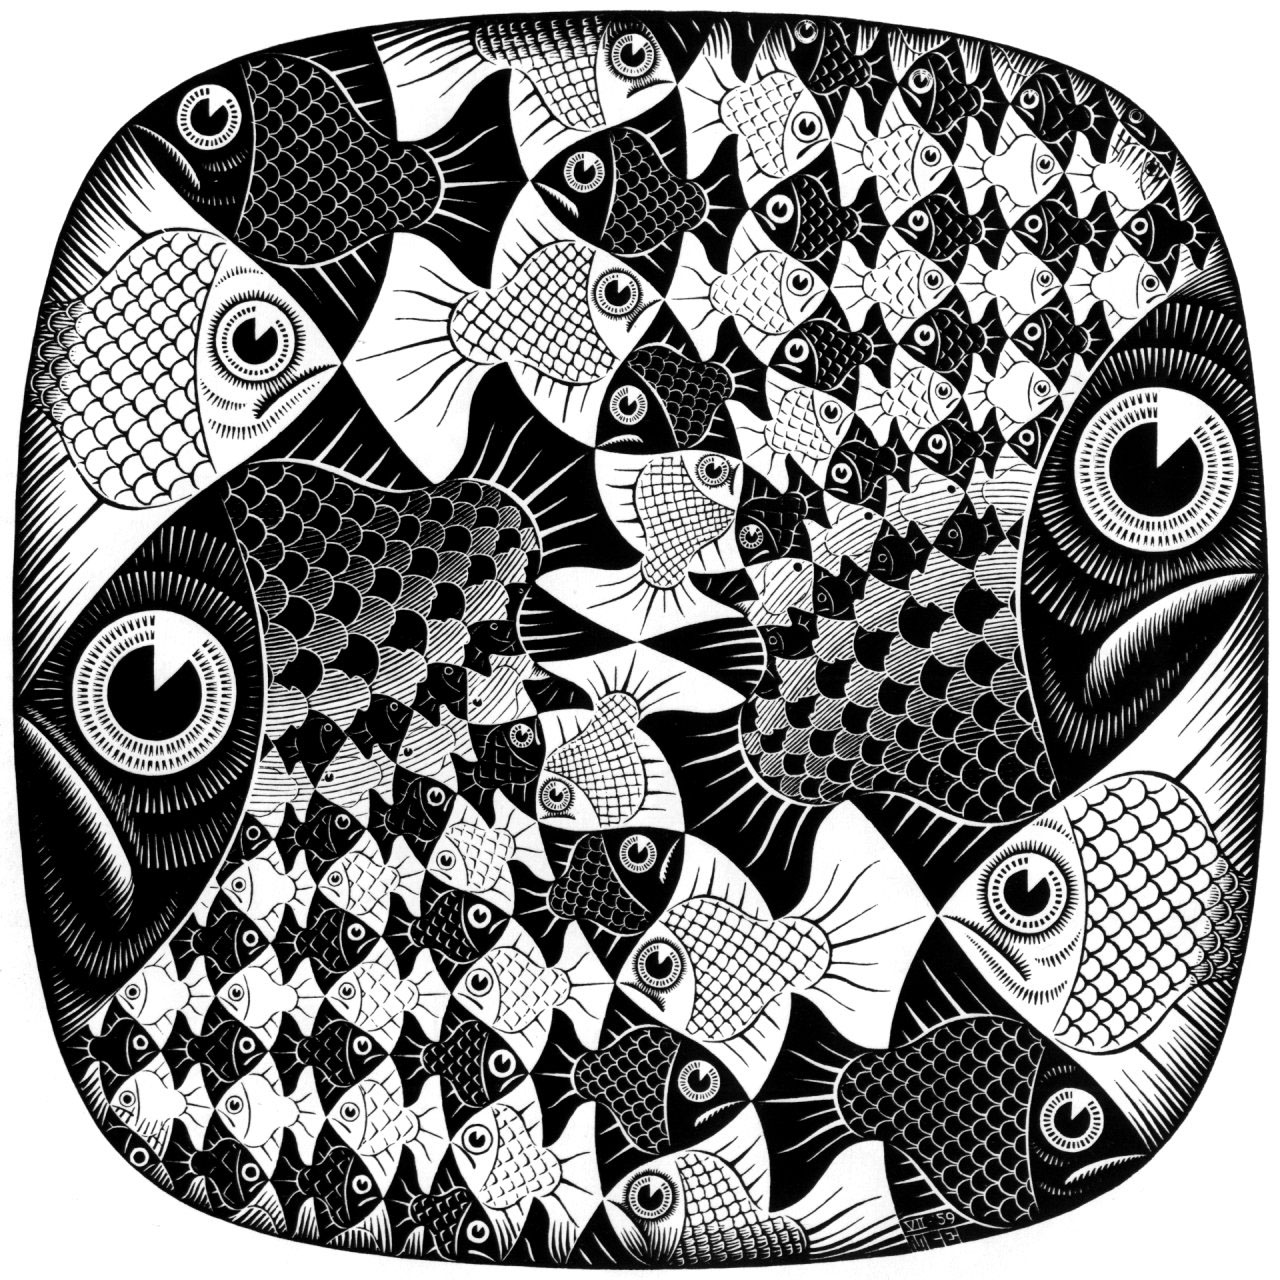
\includegraphics{img_036.jpg}
\caption[鱼和鳞,艾舍尔作。]
  {色和鳞,艾舍尔作(木刻,1959)。}
\end{figure}

一个东西的部分是这个东西自身的副本,这一想法被艾舍尔用在了他的作品中:木刻《鱼和鳞》(\fig{36})。当然,只有在足够抽象的层面上来看这些鱼和鳞时,它们才是一样的。人人都知道一条鱼的鳞并不真是这条鱼的小副本,一条鱼的细胞也不是这条鱼的小副本,然而,一条鱼的DNA(存在于这条鱼的每个细胞中)的确是整个这条鱼的一个极其复杂的“副本”——所以艾舍尔的画中的确是含有不少真理的。

所有蝴蝶的“相同之处”是什么?一个蝴蝶到另一个蝴蝶的映射并非把细胞映射到细胞,而是把功能块映射到功能块,其中,部分是宏观的,部分是微观的。映射所保持的不是功能块之间的精确比例,而是它们之间的功能关系。这就是在艾舍尔的木刻《蝴蝶》(\fig{37})中把所有的蝴蝶联系在一起的那种同构。G图中更抽象的蝴蝶也是这样,它们通过一个数学映射而联系在一起,那个映射把功能块对应到功能块,但完全不理会线条的比例、角度等等。

\begin{figure}
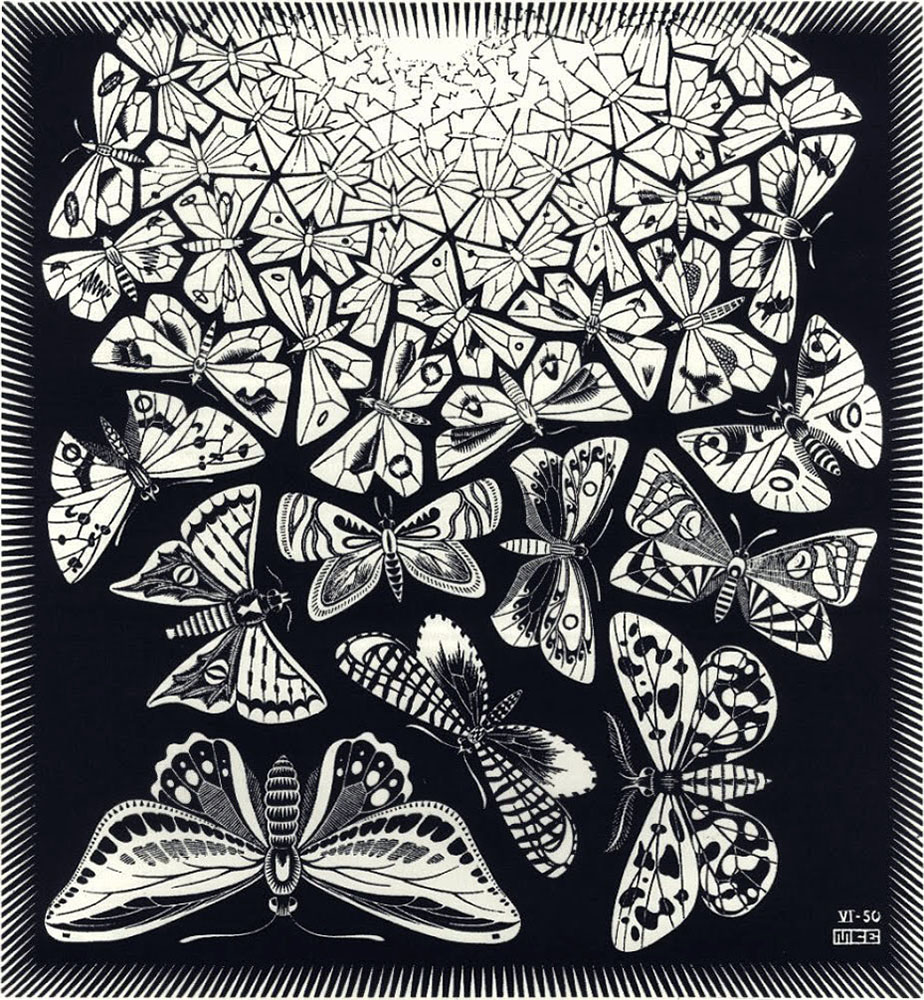
\includegraphics[width=\linewidth]{img_037.jpg}
\caption[蝴蝶,艾舍尔作。]
  {蝴蝶,艾舍尔作(木刻,1950)。}
\end{figure}

把这种对同一性的探讨提高到更为抽象的层面上,我们便可以问这样一个问题:“对于所有艾舍尔的画,这种‘同一’是在哪里?”试图在它们的片段之间寻找映射是荒谬的。令人惊异的是:即便艾舍尔作品或巴赫作品的极小的一部分也揭示出了某种同一性。就像一条鱼的DNA包含了这条鱼的每一细微末节一样,每个艺术家的“署名”也都被包含在他作品中的每一细部。我们不知该把这个叫做什么,只好说“风格”——一个模糊而难以捉摸的词。

我们会继续不断地探讨“异中之同”,以及下面这个问题:

\begin{block}
什么时候两个东西是一样的?
\end{block}
这种探讨将在本书中一再出现。我们将从各个不同的角度来提出这个问题,最终,我们会看到,这个简单的问题与智能的性质有着多么深刻的联系。

在讨论递归的一章里出现这个问题并不是偶然的,因为在递归这一领域里,“异中之同”扮演着一个中心角色。递归是以不同层次上同时出现的“同一”的事物为基础的。但在不同层次上发生的事件并不是完全相同的——确切地说,我们发现了它们中间的某种不变的特征,尽管它们在很多方面都不同。例如,在《和声小迷宫》里,所有不同层次上的故事彼此之间几乎没有什么关系——它们的“同一”仅在于两点:\pnum{1}它们都是故事,\pnum{2}它们都涉及了乌龟和阿基里斯。除此之外,它们没有一点相同之处。

\section{程序设计与递归:模块性、循环、过程}

编写计算机程序的一个基本技术,是把任务自然地分解成子任务。这要求人们看出两个过程在某种扩展了的意义上——这将导致模块性概念——是同一的。比如,某人可能想让一系列类似的操作一个接一个地执行。不必把它们都写出来,可以写一个循环,告诉计算机执行一套操作之后再回过来重新执行它们,一遍又一遍地这么做,直到某个条件被满足。循环体——要重复的那套固定指令——实际上无需完全确定,可以以某种可预知的方式有所变化。

举一个例子。一种最简单的测试自然数$N$是否是素数的方法是:一开始,把$N$用$2$除,然后用$3$、$4$、$5$等等去除,一直到$N-1$。如果$N$通过了所有这些测试,没有被整除,那么它是素数。注意,循环中的每一步都与其它步相似,却又不尽相同。还要注意,共有多少步是随N的大小而变化的——因此一个固定长的循环决不可能成为对素数性的一个一般的测试。使这个循环“终止”的准则有两个:\pnum{1}有某个数整除了$N$,这时回答“NO”并退出循环;\pnum{2}除数一直到了$N-1$,而N通过了所有测试,这时回答“YES”并退出。

于是,循环的一般想法就是:一遍又一遍地执行某些相互有关联的步骤,当遇到指定的条件时就终止。有些时候,一个循环至多有多少步预先就会知道;另一些时候,只是开动起来,等着,直到它终止。第二种类型的循环——我称之为“自由循环”——是很危险的,因为使循环终止的情况可能永远不会出现,而把计算机丢在所谓“无限循环”的状态中。有界循环与自由循环之间的差别是计算机科学中最重要的概念之一,我们将来会用一整章来讨论它:“BlooP和FlooP和GlooP”。

循环可以相互嵌套。例如,假定我们想测出$1$到$5000$之间的所有素数。我们可以再写一个循环,它一遍又一遍地使用上面描述过的测试,从$N=1$开始,到$N=5000$结束。于是我们的程序便是“循环的循环”结构。这种程序结构很典型——事实上这被认为是好的程序设计风格。这种嵌套的循环也出现在一般事务的组合指令中,以及像编织或挑花这类工作里——其中,很小的循环在较大的循环中多次重复,而后者也是重复地进行的……尽管低层循环的结果或许不过是几针,高层循环的结果却会是一大块布。

音乐中也一样,嵌套的循环经常出现——比如,一个音阶(一个小循环)在一行中出现多次,每次变一个音高。例如,在普罗科菲耶夫的《第五钢琴协奏曲》和拉赫马尼诺夫的《第二交响曲》中,最后一个乐章都包含有扩展了的小节,其中快速、中速和慢速的循环音阶同时由不同的乐器奏出,效果极好。普罗科菲耶夫的音阶是上升的,拉赫马尼诺夫的音阶是下降的。你看哪个好?

比循环更一般化的概念是“子程序”或“过程”,对之我们已略有讨论。其基本思想是把一组操作集在一起,起个名字,当做一个整体——例如花哨名词过程。我们已在RTN中看到,过程可以彼此按名字调用,借此可以简明地表示出要执行的操作序列。这是程序设计中模块化的实质所在。很明显,到处都能找到模块化现象:高保真音响系统、机械装置、生物体的细胞、人类社会——在任何有层次组织的地方。

人们常常希望让过程具有随机应变的能力。这种过程既可以窥视存储器中的东西,并选出与之相应的操作,也可以被一组明确给出的参数所控制。有时这两种方法都使用。用RTN的术语来说,所谓选择要执行的操作序列,就相当于选择走哪条通道。RTN配备了参数等设施后,就能对通道的选择进行控制了,这种增强了的递归迁移网被称为“扩充迁移网”(ATN)。如果让你按照一部由迁移网写出的语法,用一些单独的字造出有意义的——区别于无意义的——汉语句子,你大概更愿意采用ATN而非RTN。参数等设施使你能插入各种语义制约,以便防止出现像“徒劳的早饭”这种搭配不当的现象。对此我们还有许多要谈,不过要到第十八章再说了。

\section{弈棋程序中的递归}

带参数的递归程序的经典例子,是一个在下棋时每次都选择“最佳”的一步棋的程序。最佳的一步棋该是把对手置于最难受境地的一步棋。所以,检验一步棋是不是好棋的办法就是:假设你已走了这步棋,然后从你对手的角度来审视棋盘上的局面。那么你的对手会采取什么行动呢?他嘛,他要找他的最佳一步棋。也就是,他要考虑所有可能的棋步,并以在他看来是你的眼光来衡量一番,希望找出对你最为不利的走法。注意,我们现在对“最佳一步棋”的定义是递归的,就用这么一个准则:对一方来说是最好的,对另一方来说就是最坏的。寻找最佳棋步的递归过程就是这么运转,先试着走一步,然后从对手的角度调用自己!这么做的时候,它试走了下一步,于是又从对手的对手的角度调用自己——又是它自己的角度了!

这样的递归可以深入到好几层——但总是要在什么地方终了的!不向前看的话,怎么才能衡量棋局呢?这里有不少有用的准则,比如:简单地数一数各方都有多少棋子,受攻击的棋子有多少、都是什么类型的,对中路的控制,等等。以这种衡量方法为基础,递归棋步生成器就可以向上弹回到顶层,给出对不同棋步的估价。于是,自调用时必须要有一个参数指明要向前看多少步。过程的最外层调用使用这个参数的某个从外部输入的值。那之后,过程每次递归地调用自己时,它必须把它的向前看参数减少$1$。这样下去,参数达到零时,过程就转向另外的通道——即进行非递归计算。

在这一类的游戏程序中,对每一步的探索导致一棵所谓“超前搜索树”的生成,一步棋自身是树干,对方的应招是主枝,自己再应对的棋步是分枝,如此等等。\fig{38}就是一棵超前搜索树,画出了三子棋的开始棋局。当然应该想法避免彻底地探索超前搜索树的每一枝干,但这是一门艺术。在下棋情形,人——不是计算机——似乎是杰出地掌握了这门艺术。人们已经知道,第一流的棋手向前看的步数,与大多数下棋程序相比是很少的——然而人还是高明得多!计算机下国际象棋的早期阶段,有人曾估计再要十年的时间计算机(或程序)就能得世界冠军。可是,十年过去之后,计算机要成为世界冠军似乎还要再过十年……这不过是下面这个递归化的定律的又一例证:
\begin{thm}{侯世达定律}
做事所花费的时间总是比你预期的要长,即使你的预期中考虑了侯世达定律。
\end{thm}

\section{递归与不可预期性}

本章中的递归过程与前一章中的递归集是什么关系?这涉及到“递归可枚举”的概念。一个集合是r.e.的,意思是它可以通过推理规则的重复使用从一集出发点(公理)之中产生出来。这样,这个集合不断扩充,每个新的元素都是由已有的元素复合而成,就像一个“数学雪球”似的。但这恰恰就是递归的实质——定义一个东西时,使用它自己的较为简单些的版本,而非直截了当地给出它的定义。斐波那契数和卢卡斯数是r.e.集的极好例子——用一条递归规则把两个元素滚雪球式地滚成无穷的集。把一个其补集也是r.e.集的r.e.集称作“递归的”,这仅仅是个约定。

\begin{figure}
%\includegraphics{img_038.png}
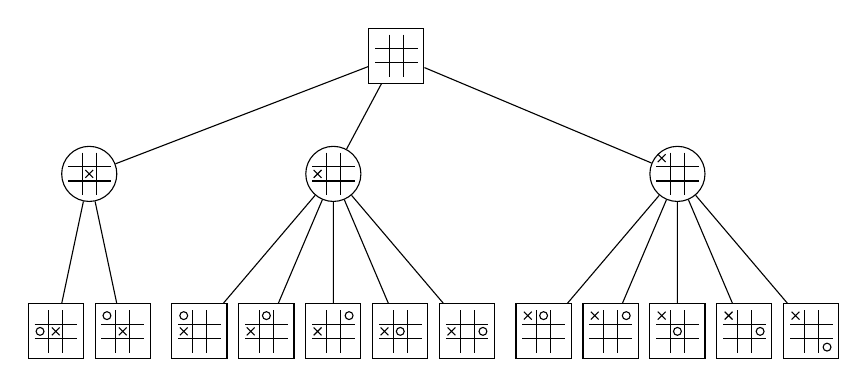
\begin{tikzpicture}[every node/.style={draw, minimum size=7mm},
  level 1/.style={level distance=15mm,sibling distance=44mm},
  level 2/.style={level distance=20mm,sibling distance=8.5mm}]
\node (O) {}
  child[xshift=5mm] { node[circle] {}
    child { node {} }
    child { node {} }
  }
  child[xshift=-8mm] { node[circle] {}
    child { node {} }
    child { node {} }
    child { node {} }
    child { node {} }
    child { node {} }
  }
  child[xshift=-8.3mm] { node[circle] {}
    child { node {} }
    child { node {} }
    child { node {} }
    child { node {} }
    child { node {} }
  };
\begin{scope}[x=.1mm, y=.1mm]
\def\GRID{%
  \draw[thin] (-27,9) -- +(54,0)  (-27,-9) -- +(54,0)
              (-9,27) -- +(0,-54) (9,27)   -- +(0,-54);}
\begin{scope}[shift=(O)]
\GRID
\end{scope}
\def\TEST#1#2{%
  \if#10\def\xs{0}\else\edef\xs{\the\numexpr#120\relax}\fi
  \if#20\def\ys{0}\else\edef\ys{\the\numexpr#220\relax}\fi}
\foreach \p / \x / \y in
  {
    O-1/0/0,
    O-2/-/0,
    O-3/-/+
  }
  {
    \begin{scope}[shift=(\p)]
    \GRID
    \TEST\x\y
    \draw plot[mark=x] coordinates{(\xs,\ys)};
    \end{scope}
  }
\foreach \p / \x / \y / \s / \t in
  {
    O-1-1/0/0/-/0,
    O-1-2/0/0/-/+,
    O-2-1/-/0/-/+,
    O-2-2/-/0/0/+,
    O-2-3/-/0/+/+,
    O-2-4/-/0/0/0,
    O-2-5/-/0/+/0,
    O-3-1/-/+/0/+,
    O-3-2/-/+/+/+,
    O-3-3/-/+/0/0,
    O-3-4/-/+/+/0,
    O-3-5/-/+/+/-
  }
  {
    \begin{scope}[shift=(\p)]
    \GRID
    \TEST\x\y
    \draw plot[mark=x] coordinates{(\xs,\ys)};
    \TEST\s\t
    \draw (\xs,\ys) circle (5);
    \end{scope}
  }
\end{scope}
\end{tikzpicture}
\caption[三子棋树。]
  {三子棋开始两步的超前搜索树。}
\end{figure}

递归枚举是个过程,其中新的东西按照一定的规则从已有的东西中产生出来。这种过程看上去似乎有许多令人惊奇的事情——比如Q序列的不可预测性。就好像那种类型的递归定义序列其行为具有内在的不断增加的复杂性,以至于走得越远,可预测性就越少。这种思想再向前推进一步,就提示我们:复杂到一定程度的递归系统,其能力可能会强有力得足够打破任何事先规定下来的模式。这不就是使智能成其为智能的性质之一吗?与其仅仅考虑由可以递归地调用自身的过程组成的程序,为什么不考虑得更复杂一些,设计出可以修改自身的程序——可以作用于程序本身,扩展、改进、推广、加固程序的程序?智能的核心之处大概就是这种“交织的递归”之所在。
